\documentclass{amsart}
\usepackage[margin=1.5in]{geometry}
\usepackage{amsmath, amssymb, amsrefs, tikz, csquotes}
\newtheorem{theorem}{Theorem}[section]
\newtheorem{lemma}[theorem]{Lemma}

\theoremstyle{definition}
\newtheorem{definition}[theorem]{Definition}
\newtheorem{example}[theorem]{Example}
\newtheorem{xca}[theorem]{Exercise}

\theoremstyle{remark}
\newtheorem{remark}[theorem]{Remark}

\numberwithin{equation}{section}

%    Absolute value notation
\newcommand{\abs}[1]{\lvert#1\rvert}

%    Blank box placeholder for figures (to avoid requiring any
%    particular graphics capabilities for printing this document).
\newcommand{\blankbox}[2]{%
  \parbox{\columnwidth}{\centering
%    Set fboxsep to 0 so that the actual size of the box will match the
%    given measurements more closely.
    \setlength{\fboxsep}{0pt}%
    \fbox{\raisebox{0pt}[#2]{\hspace{#1}}}%
  }%
}
\newcommand{\dis}{\bigsqcup}

\begin{document}
\title{Fundamental Group of Covering Spaces}

\author{Yangkun Li}
\begin{abstract}We study the connection between covering spaces and the fundamental group of base.  We will also introduce briefly some extension to the basics of this topic.\end{abstract}
\maketitle 
\section{Introduction and Preliminaries}
\noindent When studying the algebraic topology, the first example of nontrivial fundamental group one may have seen, is the the fundamental group of $S^1$, $\pi_1(S^1, x_0)$, is isomorphic to $\mathbb{Z}$. This result is achieved using tools like covering spaces and lifting correspondence. In this case, $S^1$ served as the base in a covering map. One might ask if this process is generalizable? (To some kind of covering spaces) What can we say about the fundamental group of covering spaces and how are different covering spaces related? In this paper, we will investigate these questions and derive some fundamental results.

We shall review some basic concepts first.

\begin{definition} Two paths $f$ and $f'$, mapping the interval $I = [0, 1]$ into $X$, are said to be \textbf{path homotopic} if they have the same initial point $x_0$ and the same final point $x_1$, and if there is a continuous map $F : I \times I \to X$ such that
\[
F(s, 0) = f(s) \quad \text{and} \quad F(s, 1) = f'(s),
\]
\[
F(0, t) = x_0 \quad \text{and} \quad F(1, t) = x_1,
\]
for each $s \in I$ and each $t \in I$. We call $F$ a \textbf{path homotopy} between $f$ and $f'$.

\noindent Being hotopic is an equivalance relation. We use $[f]$ to denote the equivalence class of $f$.

\noindent We assume all paths have domain $[0,1]$ for convenience.
\end{definition}

\begin{definition}If $f$ is a path in $X$ from $x_0$ to $x_1$, and if $g$ is a path in $X$ from $x_1$ to $x_2$, we define the \textbf{product of paths} $f \ast g$ of $f$ and $g$ to be the path $h$ given by the equations
\[
h(s) =
\begin{cases} 
f(2s) & \text{for } s \in \left[0, \frac{1}{2}\right], \\
g(2s - 1) & \text{for } s \in \left[\frac{1}{2}, 1\right].
\end{cases}
\]
This operation induces the \textbf{product of path homotopies} by $[f] \ast [g] = [f \ast g]$.
\end{definition}

\begin{theorem}
    Product of path homotopies is associative, has left and right inverses, and every $[f]$ has a inverse $[\overline{f}]$ by reversing the path.
\end{theorem}
\begin{definition}[Fundamental Group] Let $X$ be a topological space; let $x_0 \in X$. A path $f:[0,1] \longrightarrow X$ with $f(0) = f(1) = x_0$ is called a \textbf{loop} based at $x_0$. The homotopy class of $f$ is denoted as $[f]$. The set of path homotopy classes of loops based at $x_0$, with the operation induced by product of paths, is called the \textbf{fundamental group} of $X$ relative to the \textbf{base point} $x_0$. It is denoted by $\pi_1(X, x_0)$.
\end{definition}

\begin{definition} Let $X,Y$ be topological spaces and let $h : X \to Y$ be a continuous map with $h(x_0) = h(y_0).$ Define
\[
h_\ast : \pi_1(X, x_0) \to \pi_1(Y, y_0)
\]
by
\[
h_\ast([f]) = [h \circ f].
\]
The map $h_\ast$ is called the \textbf{homomorphism induced by $h$}, relative to the base point $x_0$.

\end{definition}

\begin{definition}[Evenly covered] Let $p : E \to B$ be a continuous surjective map. A open set $U$ of $B$ is said to be \textbf{evenly covered} (by $p$) if
$$p^{-1}(U) = \dis_{\alpha \in A} V_\alpha$$
for some collection of open sets $\{V_\alpha\}_{\alpha \in A}$ in $E$, such that for each $\alpha$, $p |_{V_\alpha}$ is a homeomorphism of $V_\alpha$ onto $U$.
\end{definition}

\begin{definition}[Covering Space and Covering maps] \label{GLCT} Let $p : E \to B$ be continuous and surjective. If there is a neighborhood $U$ for every $b \in B$ that is evenly covered by $p$, then $p$ is called a \textbf{covering map}. $E$ is said to be a \textbf{covering space} of $B$. $p$ is a \textbf{local homeomorphism} of $E$ with $B$.   
\end{definition}

\begin{theorem} [Restricting Covering Maps] \label{Restrict} Let $p : E \to B$ be a covering map. If $B_0$ is a subspace of $B$, and if $E_0 = p^{-1}(B_0)$, then the map $p_0 : E_0 \to B_0$ obtained by restricting $p$ is a covering map.

\end{theorem}

\begin{definition}[Lifting] Let $p : E \to B$ be a map. If $f$ is a continuous mapping of some space $X$ into $B$, a \textbf{lifting} of $f$ is a map $\tilde{f} : X \to E$ such that $p \circ \tilde{f} = f$. See Figure 1.
\end{definition}

\begin{figure}
    \centering
    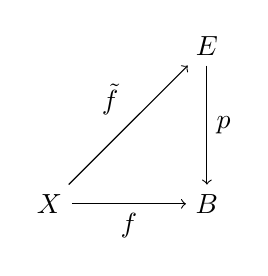
\begin{tikzpicture} [node distance=2cm, auto]
        \node (X) {$X$};
        \node (B) [right of=X] {$B$};
        \node (E) [above of=B] {$E$};
    
        \draw[->] (X) to node [swap] {$f$} (B);
        \draw[->] (X) to node {$\tilde{f}$} (E);
        \draw[->] (E) to node {$p$} (B);
    \end{tikzpicture}
    \caption{Lifting of map $f$}
\end{figure}

\begin{lemma}[Path-Lifting Lemma] \label{PLL}Let $p : E \to B$ be a covering map, let $p(e_0) = b_0$. Any path $f : [0, 1] \to B$ with $f(0) = b_0$ has a unique lifting to a path $\tilde{f}$ in $E$ with $\tilde{f}(0) = e_0$.
\end{lemma}

\begin{lemma}[Lifting of Homotopies]\label{lift homotopy} Let $p : E \to B$ be a covering map; let $p(e_0) = b_0$. Let the map $F : I \times I \to B$ be a homotopy, with $F(0, 0) = b_0$. There is a unique lifting of $F$ to a continuous map 
\[
\tilde{F} : I \times I \to E
\]
such that $\tilde{F}(0, 0) = e_0$. Furthermore, if $F$ is a path homotopy, then $\tilde{F}$ is a path homotopy.
\end{lemma}

\begin{definition}[Lifting Correspondence] Let $p : E \to B$ be a covering map and $p(e_0) = b_0$ for some $e_0 \in E$. Let $[f] \in \pi_1(B, b_0)$ and let $\tilde{f}$ be the lifting of $f$ in $E$ with $\tilde{f}(0) = e_0$. Let $\phi([f])= \tilde{f}(1)$. Then
\[
\phi : \pi_1(B, b_0) \to p^{-1}(b_0)
\]
is a well-defined set map. It is said to be the \textbf{lifting correspondence} derived from the covering map $p$. It depends on the choice of the point $e_0$. \vspace{1em}
\end{definition}

\begin{theorem} [General Lifting Correspondence Theorem] Let $p : E \to B$ be a covering map with $p(e_0) = b_0$. Then
\begin{enumerate}
    \item The homomorphism $p_\ast : \pi_1(E, e_0) \to \pi_1(B, b_0)$ is injective.
    \item Let $H = p_\ast(\pi_1(E, e_0))$. The lifting correspondence $\phi$ induces an injective map
    \[
    \Phi : \pi_1(B, b_0)/H \to p^{-1}(b_0)
    \]
    of the collection of right cosets of $H$ into $p^{-1}(b_0)$, which is bijective if $E$ is path connected.
    \item If $f$ is a loop in $B$ based at $b_0$, then $[f] \in H$ if and only if $f$ lifts to a loop in $E$ based at $e_0$.
\end{enumerate}

\end{theorem}

The details and proofs of the above lemmas and theorems can be found in Munkres' Topology \cite{mun} and Hatcher's Algebraic Topology \cite{at}. They are omitted here as this section serves as a review. It is also helpful to review some group theory facts which are not listed here, but we sometimes refer to \cite{gal}.

\section{Equivalent Covering Spaces}

\begin{definition}
    Let $p : E \to B$ and $p' : E' \to B$ be covering maps. They are said to be \textbf{equivalent} if there exists a homeomorphism $h : E \to E'$ such that $p = p' \circ h$. $h$ is called an \textbf{equivalence of covering maps}.
\end{definition}

\begin{figure}
    \centering
    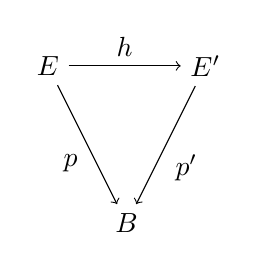
\begin{tikzpicture}[node distance=2cm, auto]
  \node (E) {$E$};
  \node (E') [right of=E] {$E'$};
  \node (B) [below of=E, xshift=1cm] {$B$};

  \draw[->] (E) to node {$h$} (E');
  \draw[->] (E) to node [swap] {$p$} (B);
  \draw[->] (E') to node {$p'$} (B);
\end{tikzpicture}
    \caption{Equivalent covering maps}
\end{figure}

\begin{remark}
    This defines and equivalence relation between covering maps since homeomorphism is an equivalence relation.
\end{remark}

\noindent For the notion of the fundamental group to make sense, we of course need the spaces $E$ and $B$ to be locally path-connected. But with this assumption, we see that it's convenient to assume $B$ is path-connected: $B$ is locally path-connected means $B$ is a disjoint union of path-components $b_i$'s. By Theorem \ref{Restrict} $p |_{p^{-1}(B_i)}$ is a covering map onto a path-connected space $B_i$. Thus we can know about $p, E$ and $B$ is the original problem by studying each set of $p |_{p^{-1}(B_i)}, p^{-1}(B_i)$ and $B_i$ without altering the idea behind the problem, for $p$ being a local homeomorphism.

Similarly, we can do this for $E$ so we assume $E$ is path-connected too. We will make this assumption for the rest of the paper unless otherwise stated.

The covering map $p$ induces an injective homomorphism (Theorem \ref{GLCT}) $p_*$ from $\pi_1(E, e_0)$ to $\pi_1(B, b_0)$. So $H_0 = p_*[\pi_1(E, e_0)]$ is a subgroup of  $\pi_1(B, b_0)$ and is isomorphic to $\pi_1(E, e_0)$. It is easy to see that $H_0$ has some sort of connection with what $p$ and $\pi_1(E, e_0)$ can be. We shall investigate this.

To do this, we first prove a generalized version of the path-lifting lemma, which allows us to lift any continuous function rather than a path.

\begin{lemma}[General Lifting Lemma] \label{GLL}Let $p : E \to B$ be a covering map with $p(e_0) = b_0$. Let $f : Y \to B$ be a continuous map, with $f(y_0) = b_0$. Suppose $Y$ is path connected and locally path connected. There exists a unique lifting $\tilde{f} : Y \to E$ of $f$ such that $\tilde{f}(y_0) = e_0$ if and only if
\[
f_\ast(\pi_1(Y, y_0)) \subseteq p_\ast(\pi_1(E, e_0)).
\]    
\end{lemma}
\begin{proof}
    \noindent We will prove this in several parts.

    \noindent We first show the if part, that is the existence and uniqueness of $\tilde{f}$.

    \begin{enumerate}
        \item To show existence of $\tilde{f}$, choose $y_1 \in Y$, there is a path $\alpha$ from $y_0$ to $y_1$ since $Y$ is path connected. Now $f \circ \alpha$ is a path in $Y$ and by path lifting lemma, we can lift $\alpha$ to a path $\gamma$ in $E$ with $\gamma(0) = e_0$. Define $\tilde{f}(y_1) = \gamma(1)$. So far we defined $\tilde{f}.$

        \item We now show $\tilde{f}$ is well defined, that is, $\tilde{f}$ is independent of choice of the path $\alpha$ in (1). Let $\alpha, \beta$ be 2 path from $y_0$ to $y_1$ in $Y$. Again let $\gamma$ be a path lifting of $f \circ \alpha$ in $E$ with $\gamma(0) = e_0$. Let $\delta$ be a path lifting of $f \circ \overline{\beta}$ in $E$ with $\delta(0) = \gamma$. Clearly $\alpha \ast \overline{\beta}$ is a loop in $Y$, so $f \circ (\alpha \ast \overline{\beta})$ is a loop in $B$. It follows that $p \circ (\gamma \ast \delta) = f \circ (\alpha \ast \overline{\beta})$ by our hypothesis $p(e_0) = b_0$. By definition this means $(\gamma \ast \delta)$ is the lifting of $f \circ (\alpha \ast \overline{\beta})$.\vspace{1em}\\
        Since $f_\ast(\pi_1(Y, y_0)) \subseteq p_\ast(\pi_1(E, e_0))$, by Theorem \ref{GLCT} (3) $\gamma \ast \delta$ is a loop in $E$ because the homotopy class of $f \circ (\alpha \ast \overline{\beta})$, $[f \circ (\alpha \ast \overline{\beta})]$, is an element of $\operatorname{im}(p_\ast)$.

        It follows that $\alpha$, $\overline{\delta}$ are liftings of $f \circ \alpha$, $f \circ \beta$ respectively, with common initial point (which is $e_0$) and end point. Thus $\tilde{f}$ is well defined.

        \item Now we will prove $\tilde{f}$ is unique. Note that if $\tilde{f}$ is a lifting of $f$, then by definition $\tilde{f} \circ \alpha$ is a lifting of $f \circ \alpha$. This is a path lifting, which is unique by Lemma \ref{PLL}, so $\tilde{f}$ must be unique.

        \item Next we prove $\tilde{f}$ is continuous. $\tilde{f}$ is clearly continuous by our construction, except at $y_1 \in Y$. We proceed by definition of continuity at this point $y_1$. For this, we will re-use the paths defined in previous parts, $\alpha$ and $\gamma$. 
        
        By assumption, let $U$ be a path connected open set containing $\tilde{f}(y_1)$ that is evenly covered by $p$. We write $p^{-1}(U) = \bigsqcup_{\alpha \in A} V_\alpha$ for open sets $V_\alpha \subseteq E$. Without loss of generality, assume that $V_0 \subset N$ for some neighborhood $N$ of $\tilde{f}(y_1)$. Then $p|_{V_0}$ is a homeomorphism.

        By continuity of $f$, there is some path-connected neighborhood $W$ of $y_1$ such that $f(y_1) \subseteq U$.

        Now for any $y \in W$, we have a path $\varphi$ from $y_1$ to $y$. Then $\alpha \ast \varphi$ is a path from $y_0$ to $y$, so $\phi = f \circ (\alpha \ast \varphi)$ is a path in $B$. By Lemma \ref{PLL} $\phi$ can be uniquely lifted to some path $\tilde{\phi}$ with $\tilde{\phi}(0) = e_0 \in E$.\\
        By construction of $\tilde{f}$ we can let $\tilde{f}(y) = \phi(1)$.

        By definition, $\operatorname{im}(f \circ \varphi) \subseteq U$, $\phi(0) = y_1$ and  we have that $p|_{V_0}$ is a homeomorphism, so the path 
        $$(p|_{V_0})^{-1} \circ f \circ \varphi$$
        is a lifting of $f \circ \varphi$ beginning at $\tilde{f}(y_1)$. But notice that the path $\gamma$ a lifting of $\alpha$ with initial point $e_0$, this means 
        $$\gamma \ast ((p|_{V_0})^{-1} \circ f \circ \varphi)$$
        is a path beginning at $e_0 \in E$ and ending at $\varphi(1) = \tilde{f}(y_1) \in V_0 \subseteq N$. Additionally, $\gamma \ast ((p|_{V_0})^{-1} \circ f \circ \varphi)$ is a lifting of $f \circ (\alpha \ast \varphi)$.

        Since $y \in W$ is arbitrary, $\tilde{f}(W) \subseteq V_0 \subseteq N$ and $W$ is a neiborhood of $y_1$, so $\tilde{f}$ is continuous at $y_1$ by definition.
    \end{enumerate}

    \noindent To prove the only if part of the lemma, simply note that $f_\ast = p_\ast \circ \tilde{f}_\ast$.
\end{proof}

Now we will use this lemma to prove a fundamental result.

\begin{theorem} Let $p : E \to B$ and $p' : E' \to B$ be covering maps with $p(e_0) = p'(e_0') = b_0$. There is a unique equivalence $h : E \to E'$ such that $h(e_0) = e_0'$ if and only if the groups
\[
H_0 = p_\ast(\pi_1(E, e_0)) \quad \text{and} \quad H_0' = p'_\ast(\pi_1(E', e_0'))
\]
are equal.
\end{theorem}

\begin{proof}
    We first prove the if part.

    Suppose $H_0$ = $H_0'$. Then we can apply the General lifting lemma to get that there exists $h: E \rightarrow E'$ such that $p' \circ h = p$ ($h$ is the lifing of $p$) with $h(e_0) = e_0'$ and $k: E' \rightarrow E$ such that $p \circ k = p'$ ($k$ is the lifing of $p'$) with $k(e_0') = e_0$. Both $h$ and $k$ are unique.

    Now notice that (see Figure 3)
    $$ p \circ k\circ h = (p \circ k) \circ h = p' \circ h = p,$$
    so $k \circ h$ is a lifting of $p$. But $\operatorname{id}E \circ p = p$ (see Figure 4), so $\operatorname{id}E$ is also the lifting of $p$. Lemma \ref{GLL} says lifting of a function is unique, so it must be the case that $k \circ h = \operatorname{id}E$.

    We can repeat the argument to show that $h \circ k = \operatorname{id} E'$ is the unique lifting of $p'$. Thus, $h$ exists and is unique, and has continuous inverse. $h$ is then an equivalence of covering spaces.
    $$$$
    Now we show the only if part. $h$ is a homeomorphism by definition, so $h_\ast(\pi_1(E, e_0)) = \pi_1(E', e_0')$ is a group isomorphism for the fundamental group is a homeomorphism invariant.

    By hypothesis we have $p' \circ h = p$, then $p'_\ast \circ h_\ast = p_\ast$ implying that 
    $$H_0' = p'_\ast(\pi_1(E', e_0')) = p'_\ast(h_\ast(\pi_1(E', e_0'))) = p_\ast(\pi_1(E, e_0)) = H_0$$
\end{proof}

\begin{figure}
    \centering
    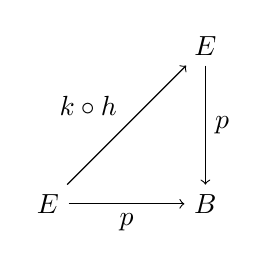
\begin{tikzpicture} [node distance=2cm, auto]
        \node (X) {$E$};
        \node (B) [right of=X] {$B$};
        \node (E) [above of=B] {$E$};
    
        \draw[->] (X) to node [swap] {$p$} (B);
        \draw[->] (X) to node {$k \circ h$} (E);
        \draw[->] (E) to node {$p$} (B);
    \end{tikzpicture}
    \caption{$k\circ h$ is the lifting of $p$}
\end{figure}

\begin{figure}
    \centering
    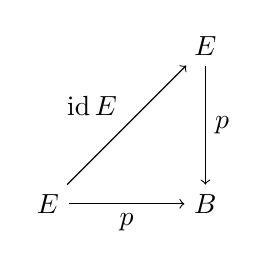
\begin{tikzpicture} [node distance=2cm, auto]
        \node (X) {$E$};
        \node (B) [right of=X] {$B$};
        \node (E) [above of=B] {$E$};
    
        \draw[->] (X) to node [swap] {$p$} (B);
        \draw[->] (X) to node {$\operatorname{id} E$} (E);
        \draw[->] (E) to node {$p$} (B);
    \end{tikzpicture}
    \caption{The identity map of $E$ is also the lifting of $p$}
\end{figure}

\noindent This theorem gives necessary and sufficient condition (in terms of fundamental groups of covering spaces) for two covering maps to be equivalent --- but the equivalence $h$ must send $e_0 \in E$ to $e_0' \in E'$.

In the case that $h$ doesn't send $e_0 \in E$ to $e_0' \in E'$, would there still be some connection between the fundamental group and the covering maps? In particular, would $h$ still be an equivalence of covering maps? Under what conditions? We shall see by studying the following theorem.$$$$
\noindent We first recall a definition from group theory.
\begin{definition}[Conjugate subgroups \footnote{We will use basic properties of conjugate subgroups without restating them. They can be found in \cite{gal}.}]
    Let $G$ be a group and let $H_1. H_2$ be subgroups of $G$. $H_1$ and $H_2$ are \textbf{conjugate} if
    $$H_2 = gH_1g^{-1} := \{gh_1g^{-1}\ | \ h_1 \in H_1\}, \text{ for some $g \in G$.}$$
\end{definition}
\begin{remark}
    Being conjugate subgroups is an equivalence relation on the collection of subgroups of $G$. The equivalence class of a subgroup is called the \textbf{conjugate class} of that subgroup.
\end{remark}

\begin{lemma} Let $p : E \to B$ be a covering map. Let $e_0$ and $e_1 \in p^{-1}(b_0)$, and let $H_i = p_\ast(\pi_1(E, e_i))$, for some indexing variable $i$ of $E$.
\begin{enumerate}
    \item[(a)] If $\gamma$ is a path in $E$ from $e_0$ to $e_1$, and $\alpha$ is the loop $p \circ \gamma$ in $B$, then $H_0$ and $H_1$ are conjugate.
    \item[(b)] Given $e_0$ a subgroup $H$ of $\pi_1(B, b_0)$ conjugate to $H_0$, there exists a point $e_1$ of $p^{-1}(b_0)$ such that $H_1 = H$.
\end{enumerate}
\end{lemma}

\begin{proof}\mbox{}
\begin{enumerate}
    \item[(a)] First, we show that $[\alpha] \ast H_1 \ast [\alpha]^{-1} \subseteq H_0$. Let $[h] \in H_1$ for some loop $h$ in $E$. Then we have $[h] = p_\ast([\tilde{h}])$ for some loop $h'$ in $E$ based at $e_1$ that is the lifting of $h$. Let $\tilde{k} = (\gamma \ast \tilde{h}) \ast \overline{\gamma}$, a loop in $E$ beginning at $e_0$. Then we have
    \begin{align*}
        p_\ast([\tilde{k}]) &= p_\ast([(\gamma \ast \tilde{h}) \ast \overline{\gamma}])\\
                            &= p_\ast([\gamma]) \ast p_\ast([\tilde{h}]) \ast p_\ast([\overline{\gamma}])\\
                            &= [\alpha] \ast [h] \ast [\overline{\alpha}]&& \text{[By definition of $\ast$ and $\alpha$]}\\
                            &= [\alpha] \ast [h] \ast [\alpha]^{-1}\\
                            &\in H_0 && \text{[By definition of $p_\ast$]}
    \end{align*}
Since $[h] \in H_1$ is arbitrary, $[\alpha] \ast H_1 \ast [\alpha]^{-1} \subseteq H_0$.

\noindent We repeat above with $\gamma$ replaced by $\overline{\gamma}$ to get $$[\overline{\alpha}] \ast H_0 \ast [\overline{\alpha}]^{-1} \subseteq H_1 \iff H_0 \subseteq [\alpha] \ast H_1 \ast [\alpha]^{-1}$$
So $[\alpha] \ast H_1 \ast [\alpha]^{-1} = H_0$, $H_0$ and $H_1$ are conjugate by definition.

\item[(b)] Let $e_0$ be given and let $H$ be conjugate to $H_0$. Then $H_0 = [\alpha] \ast H \ast [\alpha]^{-1}$ for some loop $\alpha$ in $B$ based at $b_0$. By path lifting lemma we let $\gamma$ be the lifting of $\alpha$ to a path in $E$ beginning at $e_0$ with $e_1 = \gamma(1)$. Applying (a) gives that $H_0 = [\alpha] \ast H_1 \ast [\alpha]^{-1}$, thus $H = H_1$.
\end{enumerate}
\end{proof}

\begin{theorem} \label{equiv cov}Let $p : E \to B$ and $p' : E' \to B$ be covering maps; let $p(e_0) = p'(e_0') = b_0$. The covering maps $p$ and $p'$ are equivalent if and only if the subgroups
\[
H_0 = p_\ast(\pi_1(E, e_0)) \quad \text{and} \quad H_0' = p'_\ast(\pi_1(E', e_0'))
\]
of $\pi_1(B, b_0)$ are conjugate.
\end{theorem}

\begin{proof}
    Simply apply the preceding lemma and theorem to $H_0$ and $H_0'$ gives desired result.
\end{proof}

\noindent Given $p: E \rightarrow B$ a covering map and knowing $\pi_1(B, b_0)$, Theorem \ref{equiv cov} gives us information about what $E$ should look like. Here are some examples.

\begin{example}
    We have seen that the fundamental group of the circle $S^1$ is isomorphic to the group of integers under addition. So for any covering map $p: E \rightarrow S^1$, $p_\ast(\pi_1(E, E_0))$ is a subgroup of $\mathbb{Z}$ which is abelian. But conjugate subgroups that are abelian are equal, so Theorem \ref{equiv cov} tells us that equivalent covering map of $S^1$ must send $\pi_1(E, e_0)$ to the same subgroup of $\mathbb{Z}$.

    We know from algebra classes that non-trivial subgroups of $\mathbb{Z}$ are $k\mathbb{Z} = \{kz \ | \ z \in \mathbb{Z}\}$ for some integer $k$.\footnote{This is exercise 23 on page 87 of \cite{gal}.} We also know a covering map of $S^1$\footnote{This is Example 3 of section 53 of \cite{mun}}:
    $$p: S^1 \rightarrow S^1, \quad p(z) = z^k, \ z \in \mathbb{C}, k \in \mathbb{Z}$$
    In this case we have $p_\ast(\pi_1(S^1, b_0))$ is a subgroup of $\mathbb{Z}$, which must not be non-trivial, then we see that $p_\ast$ sends the generator of $\pi_1(S^1, b_0)$ to a multiple of itself, isomorphic to the subgroup $k\mathbb{Z}$.
\end{example}

\begin{example}
    We know of another covering map of $S^1$\footnote{This is Theorem 53.1 of \cite{mun}.},
    $$p': \mathbb{R} \rightarrow S^1, \quad p'(x) = (\cos(2\pi x), \ \sin(2 \pi x))$$
    In this our covering space $\mathbb{R}$ is simply connected, having the trivial fundamental group, so $p'_\ast$ must carry $\pi_1(\mathbb{R}, x_0)$ to the trivial subgroup of $\mathbb{Z}$.
\end{example}

The above examples covers all possible subgroups of $\mathbb{Z}$, so for any other covering maps of $S^1$ other than $p, p'$, are equivalent to $p$ or $p'$.

\section{Existence of Covering Space}
\noindent The last theorem from previous section tells us that two covering maps from $E$ to $B$ are equivalent if and only if they send the fundamental group of $E$ to the same conjugacy class. Thus, we have an injective correspondence from equivalence classes of covering spaces to conjugacy classes of subgroups of $\pi_1(B, b_0)$. It is natural to ask if this correspondence is bijective. In other words, for every conjugacy class of subgroups of $\pi_1(B, b_0)$, does there there exists a unique class of equivalent covering of $B$ that corresponds to this conjagacy class. We will investigate the question in this section.

\begin{definition}
    A space $B$ is said to be \textbf{semilocally simply connected} if for each $b \in B$, there is a neighborhood $U$ of $b$ such that the homomorphism
    \[
    i_\ast : \pi_1(U, b) \to \pi_1(B, b)
    \]
induced by inclusion is trivial.
\end{definition}

\begin{remark}
    If we take a open subset of $U$ of $b$, we also get a trivial inclusion by restricting $i$ from above. So the $U$ in the above definition can be as small as needed.
\end{remark}

\begin{remark}
    Simply connected spaces are also semilocally simply path connected.
\end{remark}

We now show that the space $B$ being semilocally simple connected of is both necessary and sufficient condition for every conjugacy class of subgroups of $\pi_1(B, b_0)$ to have 
a corresponding covering space of $B$. We break the proof into two lemmas.

\begin{lemma} Let $p : E \to B$ be a covering map with $p(e_0) = b_0$. If $E$ is simply connected, then $b_0$ has a neighborhood $U$ such that inclusion $i : U \to B$ induces the trivial homomorphism
\[
i_\ast : \pi_1(U, b_0) \to \pi_1(B, b_0).
\]
\end{lemma}

\begin{proof} Suppose $U$ be a neighborhood of $b_0$ that is evenly covered by $p$. We write $$p^{-1}(U) = \bigsqcup V_\alpha.$$
WLOG let $e_0 \in V\alpha$.

Now note that for any loop $\alpha$ in $U$ based at $b_0$, it can be lifted to a loop $\tilde{\alpha}$ in $V_\alpha$ based at $e_0$ through $p|_{V_\alpha}$ (See Figure 5). Since $E$ is simply connected, $\tilde{\alpha}$ is homotopic to a constant loop. Then by Lemma \ref{lift homotopy} we can lift this homotopy to a homotopy in $B$ between $\alpha$ and a constant loop. 

Since the choices of $U$, $b$ and $\alpha$ are arbitrary $\pi_1(U, b)$ is the trivial group, thus the inclusion induce a trivial homomorphism. $B$ is semilocally simply connected by definition.
\end{proof}
\begin{figure}
    \centering
    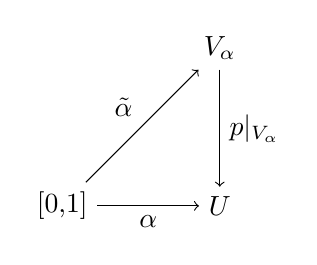
\begin{tikzpicture} [node distance=2cm, auto]
        \node (X) {[0,1]};
        \node (B) [right of=X] {$U$};
        \node (E) [above of=B] {$V_\alpha$};
    
        \draw[->] (X) to node [swap] {$\alpha$} (B);
        \draw[->] (X) to node {$\tilde{\alpha}$} (E);
        \draw[->] (E) to node {$p|_{V_\alpha}$} (B);
    \end{tikzpicture}
    \caption{Lifting of $\alpha$ to $\tilde{\alpha}$}
\end{figure}

\begin{lemma} Let $B$ be semilocally simply connected. Let $b_0 \in B$. For any subgroup $H \subseteq \pi_1(B, b_0)$, there exists a covering map $p : E \to B$ and a point $e_0 \in p^{-1}(b_0)$ such that
\[
p_\ast(\pi_1(E, e_0)) = H.
\]
\end{lemma}

The proof of this lemma is quite involved, but it captures important ideas on the construction of covering spaces. We recap some concepts from general topology first.

\begin{definition}[Quotient Map] Let $X$ and $Y$ be topological spacesand let $p : X \to Y$ be a surjective map. The map $p$ is said to be a \textbf{quotient map} if 
\begin{center}
    a subset $U$ of $Y$ is open in $Y \iff p^{-1}(U)$ is open in $X$.
\end{center}
\end{definition}

\begin{definition}[Quotient Topology] If $X$ is a topological space and $A$ is a \textit{set} and if $p : X \to A$ is surjective, then there exists exactly one topology $\mathcal{T}$ on $A$ relative to which $p$ is a quotient map. It is called the \textbf{quotient topology} induced by $p$.
\end{definition}

\begin{definition} Let $X$ and $Y$ be topological spaces. If $C$ is a compact subspace of $X$ and $U$ is an open subset of $Y$, define
\[
S(C, U) = \{f \mid f \in \mathcal{C}(X, Y)\footnote{This denotes the set of all continuous functions from $X$ to $Y$, see Chapter 7 of \cite{mun}. In \cite{mun}, $Y$ is sometimes required to have a uniform metric, likely due to the context of Chapter 7 being metric spaces. However, this requirement is not needed in general to define the compact-open topology.} \text{ and } f(C) \subseteq U\}.
\]
The sets $S(C, U)$ form a subbasis for a topology on $C(X, Y)$ that is called the \textbf{compact-open topology}.

\end{definition}

\begin{proof}
    Since we are not given the space $E$ to begin with, we need to construct everything and verify that they satisfy the desire property. Namely we need to:
    \begin{enumerate}
        \item Construct a set $E$
        \item Introduce a topology on $E$
        \item Construct a $p$ that is a covering map (which means we want to check continuity, surjectivity and evenly-covered-ness).\footnote{For this construction, really, we should also show that $E$ is path connected, because we assumed covering spaces to be path connected, but this space $E$ is constructed from merely a set. There is no guarantee on path connectedness, although $p: E \rightarrow B$ is still a covering map. In the case that $E$ is not path connected, or say even, $E$ is a disconnected space of some kind, our discussion for this whole paper would be meaningless. While the assumption can't be made, we will omit the details for that which gets into compact-open topology too much, for the sake of niceness just like why we made the assumption at the start. More details is explain by this note \cite{bha}. More on topology of functional spaces can be found here \cite{func}.}
        \item Finally we show $p_\ast(\pi_1(E, e_0)) = H.$
    \end{enumerate}
    Let us begin.
    \begin{enumerate}
        \item Let $\mathcal{P}$ be the set of all path in $B$ starting at $b_0$. Define an relation $\sim$ on $\mathcal{P}$ by $\alpha \sim \beta$ if $\alpha(1) = \beta(1).$ Note $\sim$ is an equivalence relation, and we define $E = \mathcal{P}/\sim$, equivalence classes of $\mathcal{P}$.

        \item Note that $\mathcal{P} \subseteq \mathcal{C}([0,1], B) \subseteq \mathcal{C}(\mathbb{R}, B)$. Since paths are continuous, and $[0,1]$ is a compact subset of $\mathbb{R}$, we may equip $\mathcal{C}([0,1], B)$ with the compact-open topology, then $\mathcal{P}$ has the subspace topology.

        \noindent Now we define $q: \mathcal{P} \rightarrow E$ by mapping each path to its equivalence class, then $q$ is surjective and thus induces a quotient topology on $E$.

        \item We construct $p: E \rightarrow B$ by $p([\alpha]_\sim) = \alpha(1)$, the endpoint of some path $\alpha$. Since $B$ is path connected by assumption, every point in $B$ can be the endpoint of some path thus $p$ is surjective. It remains to show that $p$ is continuous, and evenly covered-ness.

        $p$ is continuous because for every open neighborhood $U$ of $b = \alpha(1) \in B$, we have some open neighborhood of $\alpha$ by definition of compact-open topology. Then the map $q$ gives an open set in $E$ corresponding to $p^{-1}(U)$ which is open by definition of the quotient map.

        To prove evenly covered, let $b \in B$ and choose a path connected neighborhood $U$ of $B$ such that by hypothesis, $i_\ast : \pi_1(U, b) \to \pi_1(B, b)$ is trivial.  Now for every $f \in S([0,1], U)$ in the quotient topology, we have $f([0,1]) \subseteq U$. This implies that the open set $V$ in $E$ corresponding to $S([0,1], U)$ in $\mathcal{P}$ is mapped onto $U$ by $p$. Then $p^{-1}(U)$ contains $\bigcup V_i$, for some index variable $i$. Also, since $p$ $q$ are both surjective, $p \circ q$ is a surjective continuous function from $\mathcal{P}$ to $B$. Then if $p^{-1}(U)$ corresponds to some open set $S([0,1], U)$ by $p \circ q$, then there is some open set (in particular, we can represent as union of basis) $\bigcup V_i$ corresponding to both $U$ and $S_i([0,1], U)$. Moreover, $p^{-1}(U) \subseteq \bigcup V_i$. We have that $p^{-1}(U) = \bigcup V_i$. We note that this union is disjoint, for the quotient space $E$ contains unions of equivalence classes, by definition of quotient maps, and that paths that don't end at the same point do not fall into the same class.

        \item Last but not least, we show that $H = p_\ast(\pi_1(E, e_0))$. Let $\alpha$ be a loop in $B$ at $b_0$. Let $\tilde{\alpha}$ be its lift to $E$ beginning at $e_0$. Lifting Correspondence theorem tells us that $[\alpha] \in p_\ast(\pi_1(E, e_0))$ if and only if $\tilde{\alpha}$ is a loop in $E$. Now the endpoint of $\tilde{\alpha}$ is the point $[\alpha]_\sim$, and $[\alpha]_\sim = e_0$ if and only if $\alpha$ is equivalent to the constant path at $b_0$, say $c_0$, if and only if $[\alpha \ast \bar{c}_{b_0}] \in H$ (that is, they are homotopic). Note that for this to hold we must have $[\alpha] \in H$. Thus, $H = p_\ast(\pi_1(E, e_0))$
        \end{enumerate}
\end{proof}

\begin{theorem} $B$ is semilocally simple connected of if and only if every conjugacy class of subgroups of $\pi_1(B, b_0)$ to have a corresponding covering space of $B$.
\end{theorem}

\begin{proof}
    The if and only if parts are proved by \textbf{Lemma 3.5} and \textbf{Lemma 3.4} respectively.
\end{proof}

\section{Universal Covering Space}
\begin{definition}[Universal Covering Space] Let $p : E \to B$ is a covering map with $p(e_0) = b_0$. If $E$ is simply connected, then $E$ is called a \textbf{universal covering space} of $B$.
\end{definition}

The last theorem of preceding section tells us that a space $B$ has a universal covering space if and only if $B$ is path connected, locally path connected, and semilocally simply connected.

\begin{theorem} Let $p : E \to B$ be a covering map, with $E$ simply connected. Given any covering map $r : Y \to B$, there is a covering map $q : E \to Y$ such that $r \circ q = p$.
\end{theorem}
We can see that $E$ is called a \textit{universal covering space} of $B$ because it covers other covering space of $B$.

\begin{proof}
    Let $b_0 \in B$ and let $p(e_0) = b_0$ and $r(y_0) = b_0$. We apply Lemma \ref{GLL} to construct $q$. Now map $r$ is a covering map.

    Note that $E$ is simply connected, so we have
\[
p_\ast(\pi_1(E, e_0)) \subseteq r_\ast(\pi_1(Y, y_0))
\]
Therefore, there is a map $q : E \to Y$ such that $r \circ q = p$ and $q(e_0) = y_0$. By composition of covering maps, $q$ is a covering map.
\end{proof}

\[
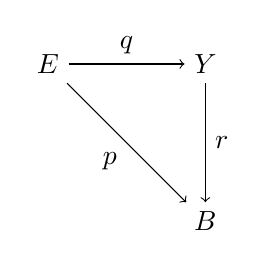
\begin{tikzpicture}[node distance=2cm, auto]
  \node (E) {$E$};
  \node (Y) [right of=E] {$Y$};
  \node (B) [below of=Y] {$B$};

  \draw[->] (E) to node {$q$} (Y);
  \draw[->] (Y) to node {$r$} (B);
  \draw[->] (E) to node [swap] {$p$} (B);
\end{tikzpicture}
\]

\section{Miscellaneous}
This section collects some results that were encountered when writing the report that aren't well-categorized due to the coverage of this paper.

\begin{definition}
    Given a covering map $p : E \to B$, equivalences of this covering space with \text{itself} are called a \textbf{covering transformations}. Composites and inverses of covering transformations are covering transformations, so this set forms a group.
\end{definition}

\begin{theorem}[Composing Covering Maps]
\textbf{Lemma 80.2.} Let $p$, $q$, and $r$ be continuous maps with $p = r \circ q$, as in the following diagram:
\begin{enumerate}
    \item[(a)] If $p$ and $r$ are covering maps, so is $q$.
    \item[(b)] If $p$ and $q$ are covering maps, so is $r$.
\end{enumerate}
\end{theorem}
\[
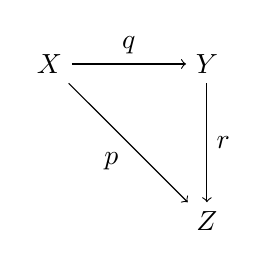
\begin{tikzpicture}[node distance=2cm, auto]
  \node (X) {$X$};
  \node (Y) [right of=X] {$Y$};
  \node (Z) [below of=Y] {$Z$};

  \draw[->] (X) to node {$q$} (Y);
  \draw[->] (Y) to node {$r$} (Z);
  \draw[->] (X) to node [swap] {$p$} (Z);
\end{tikzpicture}
\]
\section*{References}
\bibliographystyle{amsplain}
\begin{biblist}
\bib{mun}{book}{
    author={Munkres, James},
    title={Topology},
    publisher={Pearson Education Limited},
    year={2014},
    pages={326--464},
}

\bib{mar}{book}{
    author={D. Crossley, Martin},
    title={Essential Topology},
    publisher={Springer},
    year={2010}
}
\bib{at}{book}{
    author={Hatcher, Allen},
    title={Algebraic Topology},
    publisher={Cambridge University Press},
    year={2002}
}
\bib{gal}{book}{
    author={Gallian, Joseph A.},
    title={Contemporary Abstract Algebra},
    publisher={Cengage Learning },
    year={2017}
}

\bib{bha}{article}{
  author={BHATNAGAR, TEJASI},
  title={Covering Spaces},
  note={Available at \\ \text{https://math.uchicago.edu/~may/REU2017/REUPapers/Bhatnagar.pdf} }
}

\bib{func}{article}{
  author={Li, Yangkun},
  title={Function Spaces},
  note={Available at \\ \url{https://github.com/YoungkoonLi/Math-Projects/blob/main/Function\%20Spaces/MATC27_Presentation.pdf} }
}
\end{biblist}

\end{document}